%%%%%%%%%%%%%%%%%%%%%%%%%%%%%%%%%%%%%%%%%
% Short Sectioned Assignment
% LaTeX Template
% Version 1.0 (5/5/12)
%
% This template has been downloaded from:
% http://www.LaTeXTemplates.com
%
% Original author:
% Frits Wenneker (http://www.howtotex.com)
%
% License:
% CC BY-NC-SA 3.0 (http://creativecommons.org/licenses/by-nc-sa/3.0/)
%
%%%%%%%%%%%%%%%%%%%%%%%%%%%%%%%%%%%%%%%%%

%----------------------------------------------------------------------------------------
%	PACKAGES AND OTHER DOCUMENT CONFIGURATIONS
%----------------------------------------------------------------------------------------

\documentclass[paper=a4, fontsize=11pt]{scrartcl} % A4 paper and 11pt font size

\usepackage[T1]{fontenc} % Use 8-bit encoding that has 256 glyphs
\usepackage{fourier} % Use the Adobe Utopia font for the document - comment this line to return to the LaTeX default
\usepackage[english]{babel} % English language/hyphenation
\usepackage{amsmath,amsfonts,amsthm} % Math packages

\usepackage{lipsum} % Used for inserting dummy 'Lorem ipsum' text into the template

\usepackage{sectsty} % Allows customizing section commands
\allsectionsfont{ \normalfont\scshape} % Make all sections centered, the default font and small caps
\usepackage{cite}
\usepackage{listings}

%%%%%---------------------------%%%%%%%%%%%
\usepackage{fancybox}
\usepackage{graphicx}
\usepackage{pdfpages}
\usepackage{color}
\usepackage{epstopdf}
\usepackage[margin=1in, vmargin=1in]{geometry}
\usepackage{amsmath}
\usepackage{float}
\usepackage{listings}
\usepackage{verbatim}
\usepackage{booktabs}
\usepackage{tabularx}
\usepackage{longtable}
\usepackage{amsmath}
\usepackage{movie15}
\usepackage{hyperref}
\usepackage{subcaption}
\usepackage{enumerate}
\usepackage{hyperref}
\usepackage{bashful}

\usepackage{multicol}
%%%%%%%%%%%%%%---------------%%%%%%%%


\usepackage{fancyhdr} % Custom headers and footers
\pagestyle{fancyplain} % Makes all pages in the document conform to the custom headers and footers
\fancyhead{} % No page header - if you want one, create it in the same way as the footers below
\fancyfoot[L]{} % Empty left footer
\fancyfoot[C]{} % Empty center footer
\fancyfoot[R]{\thepage} % Page numbering for right footer
\renewcommand{\headrulewidth}{0pt} % Remove header underlines
\renewcommand{\footrulewidth}{0pt} % Remove footer underlines
\setlength{\headheight}{13.6pt} % Customize the height of the header

\numberwithin{equation}{section} % Number equations within sections (i.e. 1.1, 1.2, 2.1, 2.2 instead of 1, 2, 3, 4)
\numberwithin{figure}{section} % Number figures within sections (i.e. 1.1, 1.2, 2.1, 2.2 instead of 1, 2, 3, 4)
\numberwithin{table}{section} % Number tables within sections (i.e. 1.1, 1.2, 2.1, 2.2 instead of 1, 2, 3, 4)

\setlength\parindent{0pt} % Removes all indentation from paragraphs - comment this line for an assignment with lots of text

%%%%%%%%CODE INPUT STYLES%%%%%%%%%%%%%
\lstdefinestyle{BashInputStyle}{
  language=bash,
  firstline=2,% Supress the first line that begins with `%`
  basicstyle=\small\sffamily,
  numbers=left,
  numberstyle=\tiny,
  numbersep=3pt,
  frame=tb,
  columns=fullflexible,
  backgroundcolor=\color{yellow!20},
  linewidth=0.9\linewidth,
  xleftmargin=0.1\linewidth
}

\lstdefinestyle{BashOutputStyle}{
  basicstyle=\small\ttfamily,
  numbers=none,
  frame=tblr,
  columns=fullflexible,
  backgroundcolor=\color{blue!10},
  linewidth=0.9\linewidth,
  xleftmargin=0.1\linewidth
}


% settings for listings
\lstset{
    basicstyle=\scriptsize,
    numbers=left,
    numberstyle=\scriptsize,
    stepnumber=1,
    numbersep=5pt,
    showspaces=false, % don't show spaces by adding underscores
    showstringspaces=false, % don't underline spaces in strings
    showtabs=false, % don't show tabs with underscores
    frame=shadowbox,
    tabsize=4,
    captionpos=b,
    breaklines=true,
    breakatwhitespace=false,
    keywordstyle=\color{blue!70},
    commentstyle=\color{red!50!green!50!blue!50},
    rulesepcolor=\color{red!20!green!20!blue!20},
    numberbychapter=false,
    stringstyle=\ttfamily %typewriter type for strings
}
\hypersetup{
colorlinks=true,
linkcolor=black,
citecolor=black,
urlcolor=black
}

%----------------------------------------------------------------------------------------
%	TITLE SECTION
%----------------------------------------------------------------------------------------

\newcommand{\horrule}[1]{\rule{\linewidth}{#1}} % Create horizontal rule command with 1 argument of height

\title{	
\normalfont \normalsize 
\textsc{Introduction to Web Science- Fall 2014} \\ [25pt] % Your university, school and/or department name(s)
\horrule{0.5pt} \\[0.4cm] % Thin top horizontal rule
\huge Assignment Four \\ % The assignment title
\horrule{2pt} \\[0.5cm] % Thick bottom horizontal rule
}

\author{Sybil Melton} % Your name

\date{\normalsize\today} % Today's date or a custom date

\begin{document}

\maketitle % Print the title
\newpage
\tableofcontents
\listoffigures
\lstlistoflistings
\newpage
%----------------------------------------------------------------------------------------
%	TASK 1
%----------------------------------------------------------------------------------------

\section{Task One}

From your list of 1000 links, choose 100 and extract all of the
links from those 100 pages to other pages.
\\
\\
For each URI, create a text file of all of the outbound links from
that page to other URIs (use any syntax that is easy for you).
\\
\\
Upload these 100 files to github (they don't have to be in your report).

\subsection{Solution}
I chose to pick the 100 sites randomly. 
The URI to hash mappings were extracted from ``mapping.txt'' into lists
 and I used the random.randint python module to choose 100 numbers between 0 and 1000, which corresponded to the position of the URIs in the list. \cite{bib:rand}
 The already downloaded html was put into BeautifulSoup, which was able to find all of the <a href> tags and extract the links.\cite{bib:bs4}
 Each new file with the extracted links was written to a ``links'' directory.\cite{bib:files}
The 100 files are included with this report.
Listing \ref{code:links} is the python program used to open the downloaded html, extract the links with BeautifulSoup, and write them to file.  


\subsection{Python Code}
%%% Code Listing%%%%%

\lstset{
    language=python,
    caption={Link Extractor},
     label=code:links
}

\lstinputlisting{getLinks.py}
\newpage 
%----------------------------------------------------------------------------------------
%           TASK 2
%----------------------------------------------------------------------------------------

\section{Task Two}
Using these 100 files, create a single GraphViz "dot" file of the resulting graph.

\subsection{Solution}
I created a list of all the files in my ``links'' directory, which was created to hold the files from Question 1.  
Each file was opened, the original URI was extracted and labelled with the netloc from the urlparse Python module. \cite{bib:urlparse}
Then the edges were placed into adjacency lists.\cite{bib:dot}
The connected URIs were labelled with blanks, because the resulting graph has over 6000 nodes.
The graph is found in section \ref{sec:graphs}.
Originally I tried to use the URIs and then the domain names to label all the nodes, but both proved to be too long and cluttered for the graph.
Listing \ref{code:dot} is the python program used to open the links files, parse the lines, and write the ``dot'' file, which is included with this report.

\subsection{Python Code}
%%% Code Listing%%%%%
\lstset{
    language=python,
    caption={Build Dot File},
     label=code:dot
}

\lstinputlisting{getLinks.py}
\newpage
%----------------------------------------------------------------------------------------
%            TASK 3
%----------------------------------------------------------------------------------------

\section{Task Three}
Download and install Gephi.
\\
\\
Load the dot file created in \#2 and use Gephi to:
\begin{itemize}
\item visualize the graph (you'll have to turn on labels)
\item calculate HITS and PageRank
\item avg degree
\item network diameter
\item connected components \ldots
\end{itemize}	
Put the resulting graphs in your report.

\subsection{Solution}
I downloaded and used the layout scheme OpenOrd, which is advertised as scalable to up to one million nodes.
The network graph was colored by Strongly Connected ID, in order to show the node clusters and edges that connect them.
There seemed to be a lot of blog sites, so it was not surprising to see so many sites connected to wordpress.com or blogger.com.
I looked up one connection, disqus.com, and found it to be a website building company. 
So it makes sense that multilple sites would connect to it.

In Gephi, average degree was calculated to be 1.002, network diameter was 1, and connected components was 70.
The resulting graphs are in section \ref{sec:graphs}.

\subsection{Graphs}
\label{sec:graphs}
\begin{figure}[H]
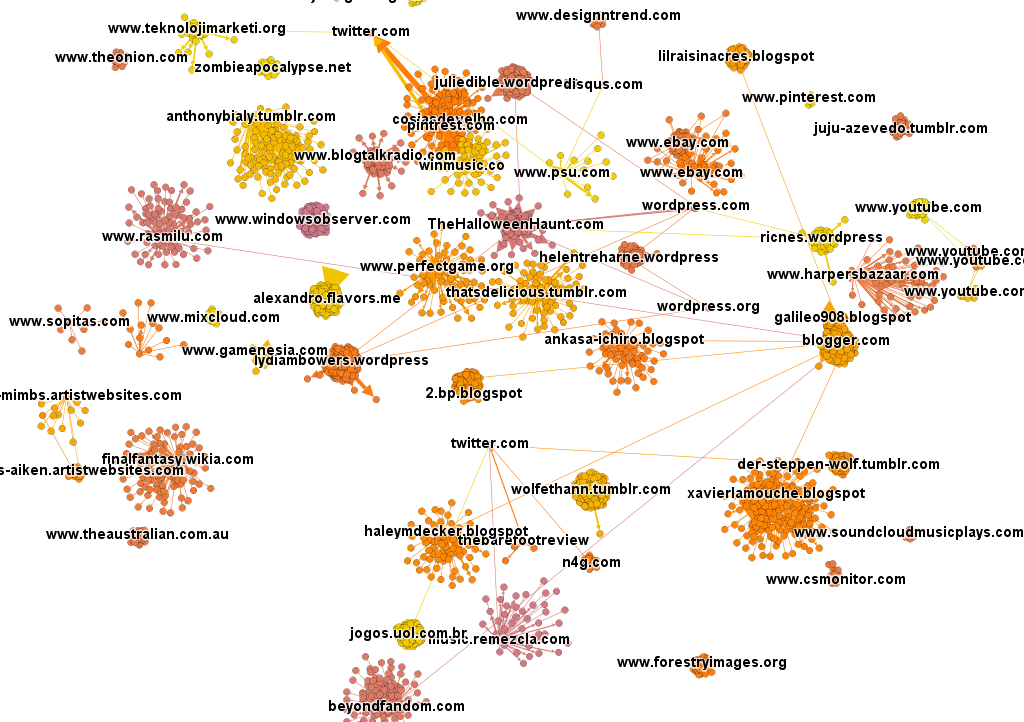
\includegraphics[width=1\textwidth]{graph1-2}
\caption{Network Graph}
\label{fig:network}
\end{figure}

\begin{figure}[H]
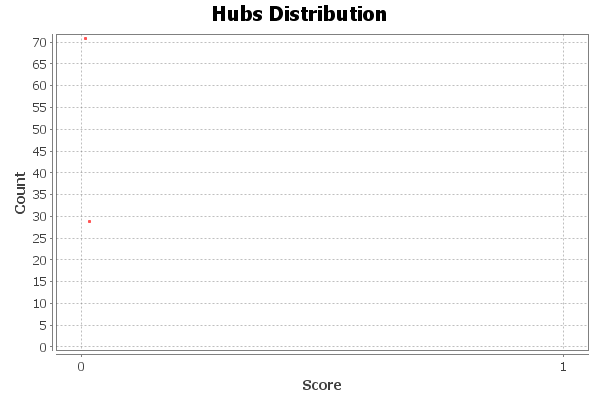
\includegraphics[width=1\textwidth]{hits/hubs}
\caption{HITS HUBS}
\label{fig:hubs}
\end{figure}

\begin{figure}[H]
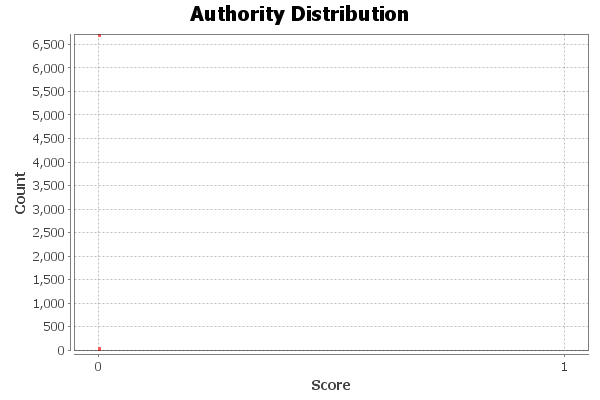
\includegraphics[width=1\textwidth]{hits/authorities}
\caption{Authorities}
\label{fig:auth}
\end{figure}

\begin{figure}[H]
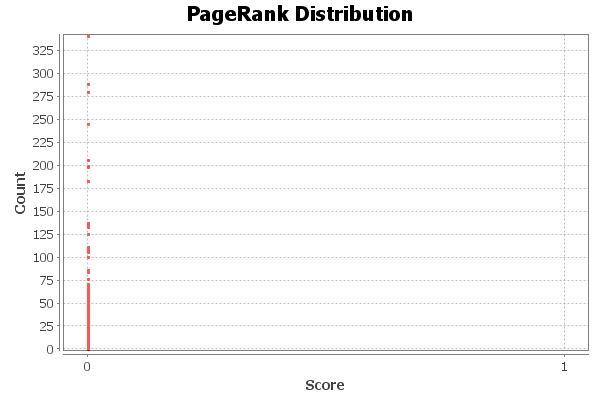
\includegraphics[width=1\textwidth]{pr/pageranks}
\caption{Page Ranks}
\label{fig:pr}
\end{figure}

\begin{figure}[H]
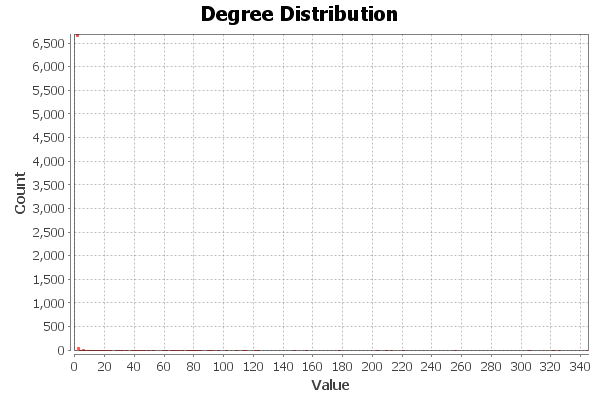
\includegraphics[width=1\textwidth]{ad/degree-distribution}
\caption{Degree Distribution}
\label{fig:degree-dist}
\end{figure}

\begin{figure}[H]
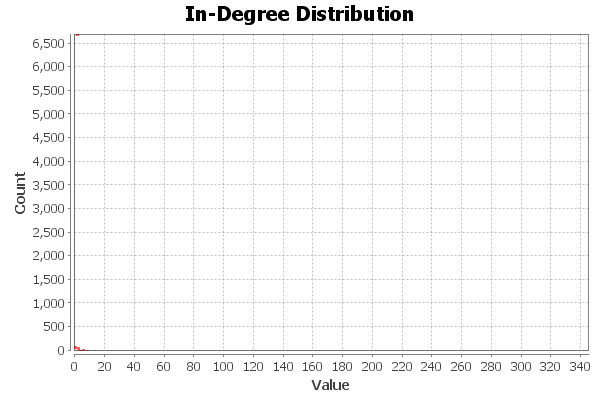
\includegraphics[width=1\textwidth]{ad/indegree-distribution}
\caption{In Degree Distribution}
\label{fig:indegree-dist}
\end{figure}

\begin{figure}[H]
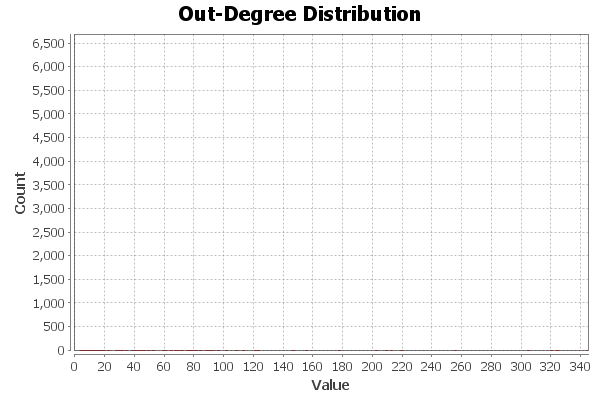
\includegraphics[width=1\textwidth]{ad/outdegree-distribution}
\caption{Out Degree Distribution}
\label{fig:outdegree-dist}
\end{figure}

\begin{figure}[H]
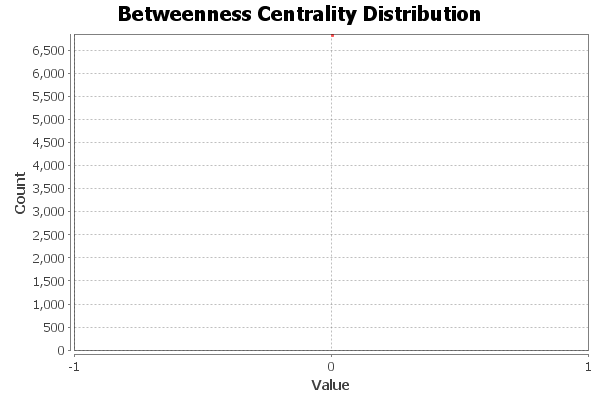
\includegraphics[width=1\textwidth]{nd/btn}
\caption{Betweenness Centrality Distribution}
\label{fig:bcd}
\end{figure}

\begin{figure}[H]
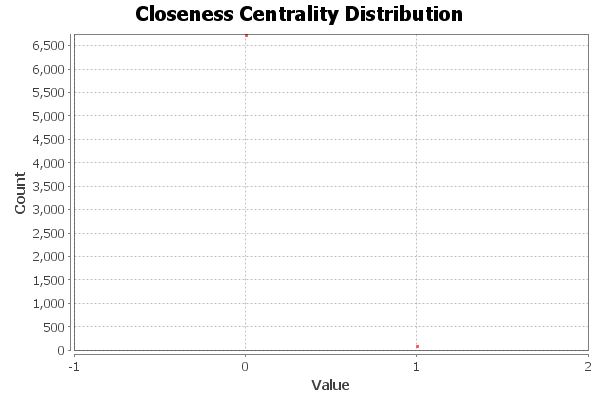
\includegraphics[width=1\textwidth]{nd/ccd}
\caption{Closeness Centrality Distribution}
\label{fig:ccd}
\end{figure}

\begin{figure}[H]
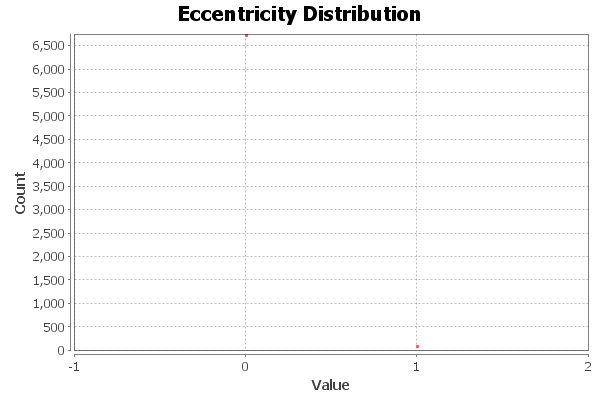
\includegraphics[width=1\textwidth]{nd/ed}
\caption{Eccentricity Distribution}
\label{fig:ed}
\end{figure}

\begin{figure}[H]
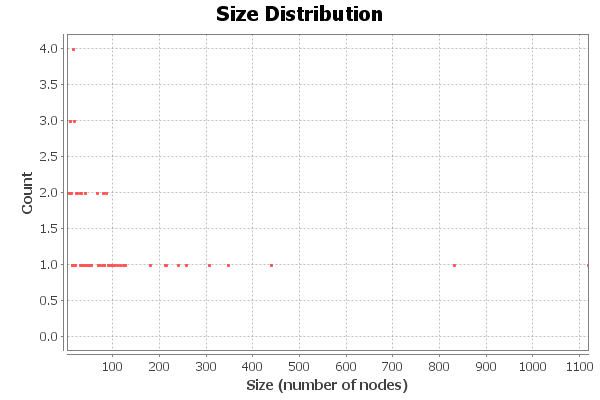
\includegraphics[width=1\textwidth]{cc/cc-size-distribution}
\caption{Connected Components Size Distribution}
\label{fig:cc}
\end{figure}

\newpage

\bibliography{references}{}
\bibliographystyle{plain}
\end{document}